\section{Browser Behaviors on HTTPS Errors}
There are many community standards for certificate validation,
    for example,
    RFC 5246, RFC 6125, and RFC 5280.
    The certificate validation in browser
    is more than a  literal replication of Internet standards protocols.
    It needs to balance security, standards, and user experiences.
\subsection{Goal and Methodology}
Our goal is to build a test harness that is able to determine whether a web browser reports HTTPS security warning for a variety of different kinds of HTTPS errors.

    Ideally, we would like to use real certificates, but doing so would require obtaining access to a real intermediate certificate(an unlikely prospect).
    Instead, we generate our own root certificate and install it so that the web browser trusts it.
    This allows us to then generate and sign intermediate and leaf certificates as we wish.
We implement out test as follows: for each test,
    (1)generates a unique DNS name,
    (2) uses OpenSSL to generate a test certificate that are syntactically(�﷨) well-formed but may violate one of the certificate constraints and internal dependencies that a valid certificate must satisfy.
    (3)generate an Nginx server configuration for the test.
Thus, each test has a dedicated DNS name and Nginx instance to serve the certificate chain.
    We create a web page to present the browser certificate validation results.
    Thus, We can record whether the HTTPS security warning is triggered by such a combination of a test certificate and a HTTPS implementation.
    In our experiment, All connections to the web server is encrypted and authenticated using TLS 1.2.

The evaluated browsers xxxxxxx

The results are summarized in Table xxx.
We experimented with different types of errors and summarized them in the table I.
\begin{table*}[htbp]
\begin{tabular}{p{2.5cm}|p{7cm}|cccc}
\hline
\multicolumn{2}{c|}{\multirow{2}{*}{HTTPS Errors}}                                                                                                                                                        & \multicolumn{4}{c}{Risk Levels of Browser Security Warnings}                             \\ \cline{3-6}
\multicolumn{2}{c|}{}                                                                                                                                                                                     & Chrome               & Firefox              & Edge                 & IE                   \\ \hline
\multirow{15}{*}{\begin{tabular}[c]{@{}c@{}}Basic Certificate \\ Validation Error\end{tabular}}     & Self-signed Certificate                                                                             & Secure               & B                    & Secure               & Secure               \\
                                                                                                    & Untrusted issuer                                                                                    & B                    & B                    & B                    & B                    \\
                                                                                                    & Incomplete Certificate Chain                                                                        & B                    & B                    & B                    & B                    \\
                                                                                                    & Expired                                                                                             & B                    & B                    & B                    & B                    \\
                                                                                                    & \multicolumn{1}{l|}{}                                                                               & \multicolumn{1}{l}{} & \multicolumn{1}{l}{} & \multicolumn{1}{l}{} & \multicolumn{1}{l}{} \\
                                                                                                    & Revoked(CRL)                                                                                        & Secure               & C                    & C                    & C                    \\
                                                                                                    & Revoked(Chrome CRLset)                                                                              & Secure               & C                    & C                    & C                    \\
                                                                                                    & Revoked(OSCP)                                                                                       & C                    & Not support          & Not support          & Not support          \\
                                                                                                    & \multicolumn{1}{l|}{}                                                                               & \multicolumn{1}{l}{} & \multicolumn{1}{l}{} & \multicolumn{1}{l}{} & \multicolumn{1}{l}{} \\
                                                                                                    & Insufficient key length (RSA512)                                                                    & B                    & B                    & B                    & C                    \\
                                                                                                    & Insufficient key length (RSA1024)                                                                   & Secure               & Secure               & Secure               & Secure               \\
                                                                                                    & Insufficient key length (ECC160)                                                                    & D                    & D                    & D                    & D                    \\
                                                                                                    & ECC256                                                                                              & Secure               & Secure               & Secure               & Secure               \\
                                                                                                    & Weak signature(SHA-1)                                                                               & B                    & B                    & Secure               & Secure               \\
                                                                                                    & Weak signature(MD5)                                                                                 & B                    & B                    & Secure               & Secure               \\ \hline
\multirow{12}{*}{\begin{tabular}[c]{@{}c@{}}Certificate Extension \\ Validation Error\end{tabular}} & Certificate chain length error                                                                      & C                    & Secure               & C                    & B                    \\
                                                                                                    & \multicolumn{1}{l|}{}                                                                               & \multicolumn{1}{l}{} & \multicolumn{1}{l}{} & \multicolumn{1}{l}{} & \multicolumn{1}{l}{} \\
                                                                                                    & endpoint certificate: no extended key usage, right key usage                                        & Secure               & Secure               & Secure               & Secure               \\
                                                                                                    & endpoint certificate: no extended key usage, wrong key usage                                        & Secure               & C                    & Secure               & Secure               \\
                                                                                                    & endpoint certificate: no extended key usage, no key usage                                           & Secure               & Secure               & Secure               & Secure               \\
                                                                                                    & endpoint certificate: right extended key usage, right key usage                                     & Secure               & Secure               & Secure               & Secure               \\
                                                                                                    & endpoint certificate: right extended key usage, wrong key usage                                     & Secure               & Secure               & Secure               & Secure               \\
                                                                                                    & endpoint certificate: right extended key usaget, no key usage                                       & Secure               & Secure               & Secure               & Secure               \\
                                                                                                    & endpoint certificate: wrong extended key usage, right key usage                                     & C                    & C                    & C                    & C                    \\
                                                                                                    & endpoint certificate: wrong extendedKeyUsage error, wrong key usage                                 & C                    & C                    & C                    & C                    \\
                                                                                                    & endpoint certificate: wrong extendedKeyUsage, no key usage                                          & C                    & C                    & C                    & C                    \\
                                                                                                    & CA certificate: key usage error                                                                     & C                    & C                    & C                    & C                    \\ \hline
\multirow{8}{*}{\begin{tabular}[c]{@{}c@{}}Name Validation\\  Error\end{tabular}}                   & no CN, right SAN                                                                                    & Secure               & Secure               & Secure               & Secure               \\
                                                                                                    & right CN, right SAN                                                                                 & Secure               & Secure               & Secure               & Secure               \\
                                                                                                    & right CN, wrong SAN                                                                                 & B                    & B                    & B                    & B                    \\
                                                                                                    & right CN, no SAN                                                                                    & B                    & C                    & C                    & C                    \\
                                                                                                    & wrong CN, right SAN                                                                                 & Secure               & Secure               & Secure               & Secure               \\
                                                                                                    & www mismatch                                                                                        & B                    & B                    & B                    & B                    \\
                                                                                                    & out-of-wildcard-scope subdomain error                                                               & B                    & B                    & B                    & B                    \\
                                                                                                    & domain name mismatch                                                                                & B                    & B                    & B                    & B                    \\ \hline
\multirow{10}{*}{\begin{tabular}[c]{@{}c@{}}HTTPS Security \\ Enhancement Error\end{tabular}}       & HPKP: private srore; first visit: wrong HPKP header, second visit: right/wrong/no HPKP header       & Secure               & Not support          & Not support          & Not support          \\
                                                                                                    & HPKP: private srore; first visit: right HPKP header right, second visit: right/wrong/no HPKP header & Secure               & Not support          & Not support          & Not support          \\
                                                                                                    & HPKP: public srore; first visit: wrong HPKP header, second visit: right/wrong/no HPKP header        & Secure               & Not support          & Not support          & Not support          \\
                                                                                                    & HPKP: public srore; first visit: right HPKP header right, second visit: right HPKP heade            & Secure               & Not support          & Not support          & Not support          \\
                                                                                                    & HPKP: public srore; first visit: right HPKP header right, second visit: wrong/no HPKP header        & B                    & Not support          & Not support          & Not support          \\
                                                                                                    & \multicolumn{1}{l|}{}                                                                               & \multicolumn{1}{l}{} & \multicolumn{1}{l}{} & \multicolumn{1}{l}{} & \multicolumn{1}{l}{} \\
                                                                                                    & HSTS: not preload list; some resouces over plain HTTP                                               & A                    & A                    & A                    & A                    \\
                                                                                                    & HSTS: not preload list; first visit: right HSTS header, second visit: HTTPS error                   & B-\textgreater{}C    & B-\textgreater{}C    & B-\textgreater{}C    & B-\textgreater{}C    \\
                                                                                                    & HSTS: not preload list; first visit: wrong HSTS header, second visit: right/wrong/no HSTS header    & Secure               & Secure               & Secure               & Secure               \\
                                                                                                    & HSTS: preload list; first visit: HTTPS errors                                                       & B-\textgreater{}C    & B-\textgreater{}C    & B-\textgreater{}C    & B-\textgreater{}C    \\ \hline
\end{tabular}
  \vspace{6pt}

\leftline{B and C represent Level B and Level C in the error warning level. "Safe" means that the browser has not detected an error and prompted a safe browsing }

\leftline{status in the indicator. "Not supported" means that the browser does not support this security policy and ignores the response header content. ECC160  }

\leftline{certificate is not supported by browsers. In HSTS Error section, ``C'' means that the policy will raise the original Level B warning to Level C (section 4.2.2).}
\end{table*}%


%\textbf{Certificate has no partial fields.}
%    A certificate may not have a Common Name or SAN field. In OpenSSL, certificates that do not fill in the above fields can also be generated and be signed.
 %   For the Common Name, some very old browsers may not support certificates without Common Name. % The Chrome browser does not support certificates without a SAN field.

\subsection{Warnings on Basic Certificate Validation Error}
Similar to the structure in the subsection3.2, the browsers behaviors are presented based on HTTPS error type.
\subsection{Warnings on Certificate Extension Validation Error}

In the experiment, we tried the KeyUsage field of various endpoint certificates, but the browser did not report the extension of the endpoint certificate. The browser will recognize the error only if the ExtendedKeyUsage is set incorrectly. For the web server, the extended usage of the endpoint certificate should be ServerAuth. If the endpoint certificate has the ExtendedKeyUsage field but does not contain the value, an error will be reported. In our experiments, the KeyUsage field was reported by the browser only if the CA certificate did not have Certificate Signing.
\subsection{Warnings on Name Validation Error}
For different error SSL certificates, we deployed a reverse proxy that passes different certificates according to SNI on the server.

The result is a certificate chain error. The error of missing the certificate is generally a warning of level B. The error setting of the intermediate certificate will result in a C level error. Certificate validation errors in revocation and extension usage errors are C-level, and other errors are B-level.

For ECC certificates, many ECC protocols in OpenSSL are not recognized by browsers. Even if the operating system can recognize it, the browser cannot establish a TLS connection through this certificate.


\subsection{Warnings on HTTPS Security-Enhancement Error}
The site's certificate must first be trusted by the browser, including server authentication and certificate/certificate chain verification. We first pin the sha256 value of the intermediate CA and any other sha256 value into the header, and the browser will cache the two sha256 values ??and verify them in the next access within the cache effective time. If the two sha256 values ??of the pin are in the same certificate chain, they will not be cached and will not prompt any errors.

If the next time the certificate issued by the site is valid and the certificate is in the pin list, the HPKP cache will be refreshed, including the SHA-256 value of the pin and the cache validity period, whichever comes first. If the intermediate CA of a certificate chain that a webmaster plans to replace is not in the current pin, you should keep using the original certificate or the alternate certificate and change the value of the other pin until the longest cache time, you can safely delete the old certificate's Pin.

In a site with HPKP cache and in effect, if the certificate received when accessing the site is a certificate in the public certificate store, and the certificate chain is not in the pin, it will be reported by the browser, but can be ignored. If the visited site is in a private certificate store, ie a self-signed certificate chain, no errors will be reported even if the certificate does not comply with the HPKP policy, and the HPKP settings cache will not be updated.

The cache of the HPKP policy has no relationship with the storage area where the certificate is located. If the certificate is legal in the browser and does not conflict with the pin in the cache, the sha256 value of the self-signed certificate chain is also stored in the pin of the HPKP policy.

When the site has the HSTS header set and is not in the preloaded list, the first visit to the site does not force https access. When the local browser has the HSTS setting cache, the browser will make a jump inside the browser when accessing the http site without initiating an HTTP network request.

\begin{figure}[htbp]
\centerline{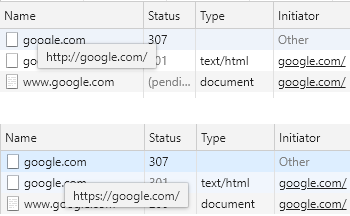
\includegraphics{Figure/fig5.png}}
\caption{Network requests to access a site with HSTS.}
\label{fig}
\end{figure}

The cache obtained by the browser through the HSTS response header is stored in the dynamic HSTS, and the site in the preloaded list is in the static storage area, which cannot be modified after the browser is compiled. However, the HSTS policy is stored in two areas and has no effect on the validity of the settings.

The HSTS policy only takes effect in the risk alert that the browser can skip. It will block the option to ignore the error, and the browser will also prompt "Cannot continue browsing due to the HSTS policy." For low-risk prompts (Level A), the browser can still access the site normally, and there will be an exclamation point prompt, which is no different from the prompt without the HSTS policy. Naturally, there is no change to the risk alert (Level C) that could not be skipped.

